\author{Marc4Prez}
\section{Epilogue}
    \begin{frame}{Epilogue}\framesubtitle{Content Overview}
        \begin{itemize}
            \item<1-> Major Choices
                %Discuss the most impactful choices during development
                %No stakeholder
                %Lorry Driver foucs --> why it didnt do shit
                %Conclusion --> Not really a lot tbh
                %SQL vs NoSQL?? Should be fairly well covered by Jesper
            \begin{itemize}
                    \item Use Case
                    \item Stakeholder 
                    \item Development Focus
            \end{itemize}
            \item<2-> Project Outcome
                %Show Enunciate
                %Ponder the use of this for developers and whether this could be released or a baseline front--end is required
                %Also consider rewards in this -> rewards for tests, rewards for front--end development, reeward for emulating > creating data provider
                %Adhering to scalability - a lot is internal development and is only recognizeable in the source code.
                \begin{itemize}
                    \item User Interface
                    \item Benefits of the Project Structure 
                    \item Scalability
                \end{itemize}
            \item<3-> Future Work
            \begin{itemize}
                \item Server \& API Improvements
                \item Additional Development
                %Consider what it would require to prepare a release worthy product, producer client for one - why?
            \end{itemize}
        \end{itemize}
    \end{frame}

    \subsection{Major Choices}
    \begin{frame}{Epilogue}\framesubtitle{Major Choices}    
        \begin{itemize}
            \item<1-> Use Case
            \begin{itemize}
                \item Military Logistic Division
                \item Lorry Drivers
                \item Postal Services
                \item Transport Services
            \end{itemize}
            %Focus here on theoretical, and why - what would be the benefit? with such benefit why did we not have one.(tried, got 1 response late on)
            \item<2-> Development Focus
            %What should be the focus for this segment? the bases should be fairly well covered, and so should why
            \begin{itemize}
                \item Data Provider
                \item Server
                \item Consumer Client
            \end{itemize}
            \item<3-> Stakeholder
            \begin{itemize}
                \item Requirements
                \item Use Case Insight
            \end{itemize}
        \end{itemize}
        \note<1-1>[item]{Initial Thoughts: Wanted to \textbf{focus} the project}
        \note<1-1>[item]{Reality: \textbf{Did not matter}}
        \note<1-1>[item]{combined with \textbf{functional and version scalability} should have provided an \textbf{easily expandable system}}
        \note<3-3>[item]{Did have the opportunity: would have delayed us and forced a \textbf{security focus}Partially why focus group}
        \note<3-3>[item]{Not having one: \textbf{Partially why focus did not matter} a lot.}
        \note<2-2>[item]{Reduced the effect of use case choice}
    \end{frame}

    \subsection{Project Outcome}
    %Maybe add a conclusion segment?? What to sum up in the conclusion would rely on covereage by the others, is there even value in this?
    \begin{frame}{Epilogue}\framesubtitle{Project Outcome}   
            \only<1>{
            Enunciate
            \begin{figure}[h]
                \centering
                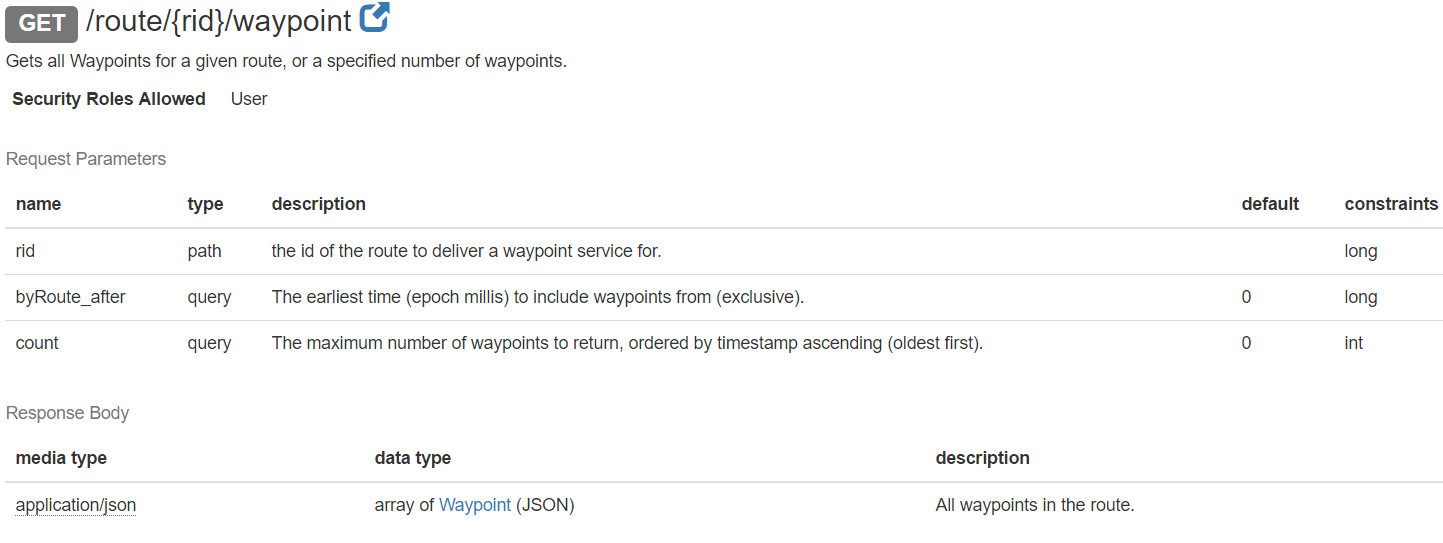
\includegraphics[scale=0.2]{images/enunciate.png}
                \caption{API documentation for a GET request.}
            \end{figure}}
            %Graphics/Show example??
            %Needs graphics, show and explain why this works as a UI for developers(can be related to IOT concept if done correct)
            \only<2>{
        \begin{itemize}
            \item Benefits of Development Strategy
            \begin{itemize}
                \item Testing
                \item Consumer Client Prototype
                \item Emulating data provider
            \end{itemize}
            
            %The rewards acquired from our development process concepts, test, Front-End Prototype, Emulating data provider over developing one
            %Tests helps us acquire code quality and the regression tests makes it easy to identify problems for further development.
            %Our load tests have given us some performance numbers, these numbers can be used to evaluate scalability for a client, laying the groundwork for a scalability analysis.
            %The few faults that exists we know why they exist because of rigerous testing(Jesper mentioned some), and aside from those we are confident that the system works, as a result of our tests running successfully.
            \item Scalability
            \begin{itemize}
                \item Scalability Testing
                %didnt do this, requires stakeholder
                \item Functional Scalability
                %Testing this would be qualitative testing which cannot really be measured, no test have been executed but this is a concept we have tried to achieve through low coupling and pattern usage
            \end{itemize}
            %Perhaps simply focus on scalability measures not related to Load Scalability - that way it also fits the theme of this segment
            %Opsummer Sass quick, evaluate - would´be evaluated upon stakeholder criteria which we do not have.
            %Framework for func scale
        \end{itemize}
        }
        \note<1-1>[item]{show stuff}
        \note<2-2>[item]{Testing acquired: \textbf{Code quality}, \textbf{Regression test}, \textbf{Reliability} useable for alter development -- refer to functional scale, we know of the few errors that exist}
        \note<2-2>[item]{Prototype gave us \textbf{User POV}, \textbf{discount stakeholder}, showing that our UI and API documentation works}
        \note<2-2>[item]{Emulate: allowed for load testing, far \textbf{quicker than development}, focus on \textbf{handling load}, rather than the ability to test \textbf{avoiding spreading too thin}}
        \note<3-3>[item]{Scalability testing(LOAD) requires stakeholder for target goal performance}
        \note<3-3>[item]{Test would be qualitative, essentially \textbf{immeasureable} -- acquired through \textbf{low coupling} and \textbf{pattern use}}
    \end{frame}

    \subsection{Future Work}
    \begin{frame}{Epilogue}\framesubtitle{Future Work}
        \begin{itemize}
            \item<1-> Server \& API Improvements
            %Additional Software Scalability(what we simply thought of as performance)
            \begin{itemize}
                    \item Adative time between requests
                    %adaptive requests --- time between requests per driver based on server traffic.
                    \item Long polling.
                    \item Sharding. %DAO, XML config, Hibernate
                    \item Expanding Services
            \end{itemize}
            \item<2-> Additional Development
            \begin{itemize}
                    \item Producer Client
                    %Necessary, library as MVP, but producer support is required
                    \item Consumer Client
                    %Not necessary
            \end{itemize}
        \end{itemize}
        \note<1-1>[item]{Adaptive time between request can \textbf{reduce server load}}
        \note<1-1>[item]{Long Polling: \textbf{Client gets notified} of new data}
        \note<1-1>[item]{Sharding: \textbf{Split information on multiple servers} this may be logical or physical, \textbf{paritcularly difficult with interval data such as spation data} and also makes everything more \textbf{complex}}
        \note<2-2>[item]{Producer client \textbf{mandatory for commercial release}, consumer client not so much}
    \end{frame}